%\documentclass[b5paper,twoside,10pt]{article}
\documentclass[b5paper,10pt]{article}

\usepackage{geometry}
         \geometry{
                 b5paper,
                 right=30mm,
                 bottom=30mm,
                 left=30mm,
                 top=30mm,
                 }

\usepackage{silence}
\WarningFilter{hyperref}{}
\usepackage{longtable}


 \usepackage{array}
\newcolumntype{P}[1]{>{\arraybackslash}p{#1}}   

\newcolumntype{L}[1]{>
{\raggedright\let\newline\\\arraybackslash\hspace{0pt}}p{#1}}

\newcolumntype{C}[1]{>{\centering\let\newline\\\arraybackslash\hspace{0pt}}m{#1}}

\newcolumntype{R}[1]{>{\raggedleft\let\newline\\\arraybackslash\hspace{0pt}}m{#1}}



\usepackage{tabularx}

\usepackage{fancyhdr}
\usepackage{pdfpages}
\usepackage{graphicx}
\usepackage{geometry}
\usepackage{xcolor}
\usepackage{wrapfig}
\usepackage{mathptmx} % Use Times New Roman font
\usepackage{setspace}
% Define a light shade of black
\definecolor{lightblack}{gray}{0.5}

\usepackage{tocloft}
\usepackage{amsmath}
\usepackage{amssymb}
\usepackage{parskip}
%\renewcommand{\cftsecfont}{\normalfont}
%\renewcommand{\cftsecpagefont}{\normalfont}
%\renewcommand{\cftsubsecfont}{\normalfont}
%\renewcommand{\cftsubsecpagefont}{\normalfont}
\renewcommand{\cftsecnumwidth}{0pt}
\renewcommand{\cftsubsecnumwidth}{0pt}
\setcounter{secnumdepth}{-1}




% Adjusting space before a new section in the table of contents
\setlength{\cftbeforesecskip}{25pt} % Adjust the value as 


\renewcommand\cftsecafterpnum{\vskip15pt}

\renewcommand\cftsubsecafterpnum{\vskip15pt}

%\usepackage[none]{hyphenrules}

\hbadness=1
\hyphenpenalty=1000



% Custom header and footer
\pagestyle{fancy}
\fancyhf{}
\renewcommand{\headrulewidth}{0pt}
\renewcommand{\footrulewidth}{0.1pt}
%\fancyhead[L]{\textcolor{lightblack}{\leftmark}} 
\fancyhead[L]{} % Research paper title
\fancyfoot[L]{\textcolor{lightblack}{\textit{Vocational Technology Education for a Sustainable Greener Economy}}}
%\fancyfoot[L]{} % Conference title
\fancyfoot[R]{\textcolor{lightblack}{\thepage}} % Page number


\newcommand{\addpaper}[4]{%
    \includepdf[pages=-, 
        addtotoc={
            1, 
            subsection, 
            1, 
            {\parindent=0.5cm \hangindent=0.5cm \hangafter=0 \capitalisewords{#1} \\ \indent \small by #2}, 
            #4
        },
        pagecommand={\thispagestyle{fancy}}
    ]{#3}
}


\usepackage{mfirstuc}
\MFUnocap{a}
\MFUnocap{an}
\MFUnocap{the}
\MFUnocap{at}
\MFUnocap{by}
\MFUnocap{for}
\MFUnocap{in}
\MFUnocap{of}
\MFUnocap{on}
\MFUnocap{to}
\MFUnocap{up}
\MFUnocap{with}
\MFUnocap{and}
\MFUnocap{but}
\MFUnocap{nor}
\MFUnocap{or}
\MFUnocap{so}
\MFUnocap{yet}

\MFUnocap{are}
\MFUnocap{or}
\MFUnocap{etc}
\MFUnocap{out}
\MFUnocap{as}
\MFUnocap{over}

\MFUnocap{across}






% Define the macro
\newcommand{\sessiontitle}[2]{
    \newpage % Start a new page
   % \thispagestyle{empty} % Optional: Remove the page number
    \begin{center}
        \vspace*{0.35\textheight}% Vertically center the text
        \Large \bfseries \textsc {#1}\\
        \vspace{1cm}
          \LARGE \bfseries \textsc {#2}
        \vspace*{\fill}
    \end{center}
    \addcontentsline{toc}{section}{\textsc{#1 - #2}}
    \newpage % Start a new page after the section title
}




\usepackage[hidelinks]{hyperref}

% \usepackage[colorlinks=true, linkcolor=blue, urlcolor=blue, citecolor=blue]{hyperref}




\renewcommand{\contentsname}{\begin{center}\textsc{ Table of Contents}\end{center}}

% Title of the document
\title{}
\author{}
\date{}



\usepackage{eso-pic}
\usepackage{tikz}
%\usepackage{hyperref}
%\usepackage{pgfplots}
\usepackage{transparent}




 

%\newcommand{\tocbutton}{\hyperlink{toc}\fbox{{\textit{\footnotesize{Click here to Return to the table of Contents}}}}}
%\fancyhead[R]{\tocbutton}










%%%%%%%%%%%%%%%%%%%%%%%%%%%%%%%%%%%%%%%%%%%%%%%%%%%%%%%%%%%%%%

\begin{document}

\newgeometry{
    right=0mm,
    bottom=0mm,
    left=0mm,
    top=0mm,
}

\thispagestyle{empty} % Remove page number
\begin{figure}[ht]
    \centering
    
\includegraphics[width=\paperwidth, height=\paperheight, keepaspectratio]{Images/Front.jpeg}
\end{figure}
\newpage


        
\newgeometry{
    right=15mm,
    bottom=15mm,
    left=15mm,
    top=15mm,
}


\begin{titlepage}
    \centering
    
\includegraphics[width=0.2\textwidth]{Images/Logo.jpeg}\par\vspace{1.5cm}
    {\scshape\LARGE International Research Symposium - 2024 \par}
    {\scshape\Large (IRS 2024-UoVT)\par}
    \vspace{2.5cm}
    {\huge  Vocational Technology Education for a Sustainable Greener Economy \par}
    \vspace{2cm}
    
\includegraphics[width=0.2\textwidth]{Images/Unilogo.png}\\
    \vspace{2.5cm}
    {\Large University of Vocational Technology\par}
    %\vspace{0.5cm}
    {\Large Sri Lanka\par}
    \vfill
    {\large December 2024\par}

    % You can add more details here if needed
\end{titlepage}
\restoregeometry
\setcounter{page}{1}
\pagenumbering{Roman}


\vspace*{1cm}
\begin{center}
    \LARGE{\textsc{\textbf{Book of Abstracts}}}\\ \vspace{1cm}
    \Large{International Research Symposium - 2024}\\ \vspace{0.5cm}
    IRS 2024 - UoVT
\end{center}
\vspace{1cm}
\textbf{DISCLAIMER}\\ 

ISSN 2602-8778: \textcopyright \, University of Vocational Technology\\


The papers published in these proceedings reflect the opinion of the respective authors.
Information contained in these proceedings has been obtained by the editors from sources
believed to be reliable. Authors of specific papers are responsible for the accuracy of the text
and technical data. Neither the publisher nor the editors guarantee the accuracy or completeness
of any information published herein, and neither the publisher nor the editors shall be
responsible for any errors, omissions, or damages arising out of use of this information.
Trademarks are used with no warranty of free usability.

All rights reserved. No part of this publication, including the cover design, may be reproduced,
stored or transmitted in any form or by any means, whether electrical, chemical, mechanical,
optical, recording or photocopying, without prior permission of the publisher.



\newpage
% Front page without margins
% \newgeometry{top=0cm, bottom=0cm, left=0cm, right=0cm}
% \begin{center}
% 	
\includegraphics[width=\paperwidth, height=\paperheight]{Images/Front.png}
% \end{center}
% \restoregeometry

%\clearpage
% Start page numbering from this page

% Table of Contents

\addcontentsline{toc}{section}{\textsc{Table of Contents}}
%\setlocalecaption{english}{contents}{Table of Contents}
%\hypertarget{toc}{}
\tableofcontents
\newpage

\sessiontitle{Proceedings of IRS 2024}{Preambles}\newpage



 



% Chairman's message page

\thispagestyle{fancy}
	
	\vspace{-2em} % Adjust vertical space as needed
	\begin{center}



\addcontentsline{toc}{subsection}{List of Reviewers}    
\subsection*{\textsc{List of Reviewers}}
	\end{center}
\vspace{1cm}
\onehalfspacing
%\subsubsection*{intenal supervisors}
\begin{longtable}{ L{4.8cm}  L{6.5cm} }  

    %\rule{0pt}{3ex}
    Prof. Ayantha Gomes & Sri Lanka Institute of Information Technology\\
Prof. W.A.L. C. Waliwita & Gampaha Wickramarachchi University of Indigenous Medicine\\
Dr. Ruvan Abeysekara & BCAS Campus\\
Prof. Chandana Jayalath & University of Vocational Technology\\
Prof. Ravindra Koggalage & University of Vocational Technology\\
Dr. Subodha Muhandiram & Vorarlberg University of Applied Sciences\\
Dr. Dayani Nayantha Kahagala Hewage & GHD Pty Ltd\\
Dr. Sanjaya Thilakarathne & University of Colombo\\
Dr. Shashinie M. Thenabadu & University of Colombo\\
Dr. Nayana Amarawickrama & University of Colombo\\
Dr. Buddhika Samarasekara & University of Sri Jayewardenepura\\
Dr. Ravimal Bandara & University of Sri Jayewardenepura\\
Dr. P.B.S.L. Pushpakumara & University of Sri Jayewardenepura\\
Dr. Chathuri Senanayake & University of Sri Jayewardenepura\\
Dr. Mihiri Munasinghe & University of Sri Jayewardenepura\\
Dr. Lochandaka Ranathunga & University of Moratuwa\\
Dr. Nalaka Jayantha & University of Moratuwa\\
Dr. Pasan Henadeera & University of Moratuwa\\
Dr. Prasanna Illankoon & University of Moratuwa\\
Dr. Sumith Gopura & University of Moratuwa\\
Dr. Chamod Hettiarachchi & University of Moratuwa\\
Dr. Kaushalya Wijayasekara & University of Ruhuna\\
Dr. Iromi Ranaweera & University of Ruhuna\\
Dr. Niranjan Kannangara & University of Ruhuna\\
Dr. Chamila Dias & Open University of Sri Lanka\\
Dr. Shakila Pathirana & University of Kelaniya\\
Dr. D. Ashoka Kumara & General Sir John Kotelawala Defence University\\
Dr. Wijendra Gunathilaka & General Sir John Kotelawala Defence Univesity\\
Dr. N.S.D.Madugodage & Buddhist and Pali University of Sri Lanka\\
Dr. R.M.S.N.Embogama & University of the Visual and Performing Arts\\
Dr. T.M.A.P.Thennakoon & Sri Lanka Institute of Advanced Technological Education\\
Dr. K.M.S.K.Karunarathne & Sri Lanka Institute of Advanced Technological Education\\
Dr.(Mrs.) Renuka Perera & Gampaha Wickramarachchi University of Indigenous Medicine\\
Dr. M.W.P. Maduranga & Sri Lanka Technology Campus\\
Dr. Janaka Jayalath & Tertiary and Vocational Education Commission\\
Dr. Priyantha Bandara & Sri Lanka Institute of Information Technology\\
Dr. Nialnthi Fernando & NERD Center\\
Dr. L.W.Sunil Kularatne & University of Vocational Technology\\
Dr. U.A.S.K. Edirisinghe & University of Vocational Technology\\
Dr. D.D.D  Suraweera & University of Vocational Technology\\
Dr. Jayalal Wettasinghe & University of Vocational Technology\\
Dr. Kasun Nandapala & University of Vocational Technology\\
Dr. Sanjeewa Sondarangallage & University of Vocational Technology\\
Dr. S.A.N. Danushka & University of Vocational Technology\\
Dr. J.A.E.C.  Jayawardena & University of Vocational Technology\\
Dr. Thikshani Somarathna & University of Vocational Technology\\
Mr. S.L. Priyantha Fonseka & University of Peradeniya\\
Mrs. E.W.Biyiri & Rajarata University of Sri Lanka\\
Mr. Rasika Jayasinghe & University of Sri Jayewardenepura\\
Ms. Lakmini Kalugampitiya & University of Sri Jayewardenepura\\
Mr. Reshan Perera & University of Moratuwa\\
Ms. Chandi Karunarathna & Uva Wellassa University\\
Ms. W.N. Kawmudi & General Sir John Kotelawala Defence Univesity\\
Mr. Vijayanathan Senthooran & University of Vavuniya\\
Mr. T. Arudchelvam & Wayamba University of Sri Lanka\\
Ms. V.K.N. Kurukulaarachchi & CINEC Campus\\
Dr. Harsha Jayakody & Ministry of Health\\
Mr. H.M.Somaratne & University of Vocational Technology\\
Ms. Sumali Morapitiya & Institute of Technology, University of Moratuwa\\
Mr. Mangala Silva & Synergo Consultants (Pvt.) Ltd.\\
Mr. Ruchira Abeyweera & Open University of Sri Lanka\\
Ms. Samindi Perera & General Sir John Kotelawala Defence University\\
Mr. Sudheera Mathakadheera & John Keels Holdings\\
Ms. K.G. Alahapperuma & University of Vocational Technology\\
Ms. J.K. Kanthi & University of Vocational Technology\\
Mr. S.P.A.R.S. Jayathilaka & University of Vocational Technology\\
Mr. Dilantha Rathnayake & University of Vocational Technology\\
Mr. D.T. Ganegoda & University of Vocational Technology\\
Mr. P. Uruthiran & University of Vocational Technology\\
Ms. Y.S.Manathunga & University of Vocational Technology\\
Ms. L.H.D.L. Ranasuriya & University of Vocational Technology\\
Ms. R.M.P.Seneviratne & University of Vocational Technology\\
Ms. W.A.I.M.Gunasekara & University of Vocational Technology\\
Mr. H.P.A.I. Pathirana & University of Vocational Technology\\
Ms. P.M  Perera & University of Vocational Technology\\
Ms. Malkanthi Thenabadu & University of Vocational Technology\\
Ms. U. Sivachelvy & University of Vocational Technology\\
Mr. T.D. Denagama & University of Vocational Technology\\
Ms. G.M.S.R.G.Manawadu & University of Vocational Technology\\
Ms. J.A.M.B.Karunarathna & University of Vocational Technology\\
Ms. A.A.Gunawardana & University of Vocational Technology\\
Mr. D. Premarathna & University of Vocational Technology\\
Ms. B.M.T.D. Jayasekara & University of Vocational Technology\\
Ms. K.G.N.P. Rajapaksha & University of Vocational Technology\\
Mr. H.A.G. Madushanka & University of Vocational Technology\\
Mr. H.N.W. Gunasekara & University of Vocational Technology\\
Mr. S.V.R.Gamage & University of Vocational Technology\\
Ms. A.A.S.U  Gunarathne & University of Vocational Technology\\
       
        
\end{longtable}    
\newpage
\singlespacing

\thispagestyle{fancy}
	
	\vspace{-2em} % Adjust vertical space as needed
	\begin{center}



\addcontentsline{toc}{subsection}{Editorial Committee}    
\subsection*{\textsc{Editorial Committee}}
	\end{center}
\vspace{1cm}
\onehalfspacing
%\subsubsection*{intenal supervisors}

\begin{longtable}{ L{4.8cm}  L{6.5cm} } 

     Dr. Kasun Nandapala & Director - Admission, Accreditation \& Quality Assurance \\

      Mr. T.D. Denagama & Head, Department of Construction Technology \\

        Ms. W.A.I.M. Gunasekara & Head, Department of Industrial Management \\

       Ms. L.H.D.L. Ranasuriya & Head, Department of Language Studies \\

    Ms. Y. S. Manathunga & Head, Department of Education \& Training \\

     Mr. P.H.S.S. Wijayarathna & Head, Department of Network Technology \\
      
     Dr. (Ms.) J.A.E.C. Jayawardena & Acting Head, Department of Agriculture \& Food Technology \\


   

   

     
    Mr. P Uruthiran & Acting Head, Department of Software Technology \\

   


     Prof. Chandana Jayalath & Professor, Department of  Quantity Surveying \\

     Dr. D.D.D. Suraweera  & Senior Lecturer, Department of Electro-Mechanical Technology\\

     Dr. J.A.D. Jayalath & Senior Lecturer, Multimedia \& Web Technology \\

     Dr. (Ms.) T. Somaratne & Senior Lecturer, Department of Agriculture \& Food Technology \\

       Ms. A.A. Gunawardana & Senior Lecturer, Department of Language Studies \\

         Ms. J.A.M.B. Karunarathna & Senior Lecturer, Department of Language Studies \\

          Ms. W.C.C. Sumathiratna & Senior Lecturer, Department of Building Services Technology \\


           Ms. K.G. Alahapperuma & Senior Lecturer, Department of  Electro-Mechanical Technology \\

             Ms. J.K. Kanthi & Senior Lecturer, Department of  Electro-Mechanical Technology \\

             Ms. M. Thenabadu & Senior Lecturer, Department of Agriculture \& Food Technology \\

         Ms. U. Sivachelvy & Senior Lecturer, Department of Industrial Management \\

             Ms. B.M.T.D. Jayasekara & Senior Lecturer, Department of Industrial Management \\

    

     

   

     

    
             Ms. K .T. P. C. Somarathna & Lecturer (Probationary), Department of Language Studies \\
     
          Ms. A.A.S.U. Gunarathna & Lecturer (Probationary), Department of Construction Technology \\
      

      

      Mr. P.D.S. Ashan & Lecturer (Probationary), Department of Building Services Technology \\

         Mr. H.A. Gayan Madushanka & Lecturer (Probationary), Department of Film \& Television Production Technology \\

    
         Mr. H.N.W. Gunasekara & Lecturer (Probationary), Department of Electro-Mechanical Technology \\

         Mr. A.H.M.S. Siriwardana & Lecturer (Probationary), Department of Construction Technology \\

         Mr. G.A.N. Sampath & Lecturer (Probationary), Department of Film \& Television Production Technology \\

        Mr. S.V.R. Gamage & Lecturer (Probationary), Department of  Electro-Mechanical Technology \\

         

           Mr. L.P.S.S. Dissanayake & Lecturer (Probationary), Department of  software Technology \\

          

       

       

          

         

            
             

          

            

               Dr. S.A.N. Danushka & Teaching Assistant, Department of Education \& Training \\

             Ms. T.R. Vidanapathirane & Teaching Assistant, Department of Industrial Management \\

             

             

            
            
   

    
    
   
    
   
   
   
    
   
    
  
\end{longtable}



\newpage
\singlespacing

\thispagestyle{fancy}
	
	\vspace{-2em} % Adjust vertical space as needed
	\begin{center}



\addcontentsline{toc}{subsection}{Symposium Organizing Committee}    
    \subsection*{\textsc{Symposium Organizing Committee}}
	\end{center}
\vspace{1cm}
\onehalfspacing
\subsubsection*{Advisory Committee}


\begin{longtable}{ p{4.8cm}  p{6.5cm} } 
  
    Professor C. Mahesh Edirisinghe  & Vice Chancellor   \\
    Dr. D.D.D. Suraweera  & Former Chair – IRS 2017 \\
    Prof. Chandana Jayalath & Former Chair – IRS 2021 \\
    Dr. L.W.S. Kularatne & Former Chair – IRS 2022 \\
    Mr. H.A. Seneviratne & Former Chair – IRS 2023 \\
\end{longtable} 

\subsubsection*{Programme Committee}

\begin{longtable}{ L{4.8cm}  L{6.5cm} } 
    %\rule{0pt}{3ex}
   
    Ms. P.M Perera & Symposium Chair \\
    Ms. Samantha Manawadu & Symposium Co-Secretary \\
    Mr. R.R.M.D.P Rathnayake & Symposium Co-Secretary \\
    % Dr. L.W.S Kularatne & Dean, Faculty of Education \\
    Ms. T.K Malwatte & Dean, Faculty of Information Technology \\
    Dr. Jayalal Wettasinghe & Dean, Faculty of Engineering Technology \\
    Dr. U.A.S. Kamal Edirisinghe & Dean, Faculty of Industrial Technology \\
    Dr. Kasun Nandapala & Director - Admission, Accreditation and Quality Assurance \\
    Mr. S.P.A.R.S. Jayathilaka & Director - Human Resource Development Centre \\
    Mr. A.M.C.K. Gunathilaka & Director - Media \& Information Services \\
    Ms. Dilini Ranasuriya & Head, Department of Language Studies \\
    Ms.Y.S Manathunga & Head, Department of Education \& Training \\
    Ms. Indrachapa Gunasekeara & Head, Department of Management Studies \\
    Ms. S.R.M.P. Seneviratna & Head, Department of Quantity Surveying \\
    Mr. D.T. Ganegoda & Head, Department of Electro Mechanical Technology \\
    Mr. T.D. Denagama & Head, Department of Construction Technology \\
    Dr. (Ms.) J.A.E.C. Jayawardena & Acting Head, Department of Agriculture \& Food Technology \\
    Mr. R.M.C.A.B Rathnayake & Acting Head, Department of Network Technology \\
    Mr. P. Uruthiran & Acting Head, Department of Software Technology \\
    Ms. S.G. Nambuwasam & Acting Head, Department of Multimedia \& Web Technology \\
    Professor R.L.W Koggalage & Associate Professor, Department of Electro Mechanical Technology \\
    Dr. S.D.A Sanjeewa & Senior Lecturer, Department of Electro Mechanical Technology \\
    Dr. Janaka Jayalath & Senior Lecturer, Multimedia \& Web Technology \\
    Dr. (Ms.) T. Somaratne & Senior Lecturer, Department of Agriculture \& Food Technology \\
    
    Dr. S.A.N. Danushka & Teaching Assistant, Department of Education \& Training \\
    Mr. M.G. Dharmasiri & Director General (Covering) / Senior Assistant Registrar (Establishments and Administration) \\
    Mr. R.D.P.I. Priyadarshana & System Administrator \\
    Mr. T.C. Jayamuthuge & Producer \\
\end{longtable}



\newpage
\singlespacing

\onehalfspacing




\thispagestyle{fancy}
	
	%\vspace{-2em} % Adjust vertical space as needed
% 	\begin{center}



% \addcontentsline{toc}{subsection}{Message of the Vice Chancellor}    
% \subsection*{\textsc{Message of the Vice Chancellor}}
% 	\end{center}

   
    
%     \begin{wrapfigure}{l}{0.3\textwidth}
% 		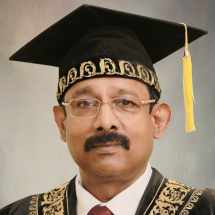
\includegraphics[width=0.3\textwidth]{Images/VC.png}
% 	\end{wrapfigure}
	%\vspace{2em} % Adjust vertical space as needed

\addmessage{Vice Chancellor}{VC.png}


	
	
	Welcome to the International Research Symposium 2023. We are delighted to have you here and look forward to an engaging and productive event. 
	
	Welcome to the International Research Symposium 2023. We are delighted to have you here and look forward to an engaging and productive event. Welcome to the International Research Symposium 2023. We are delighted to have you here and look forward to an engaging and productive event. Welcome to the International Research Symposium 2023. We are delighted to have you here and look forward to an engaging and productive event. Welcome to the International Research Symposium 2023. We are delighted to have you here and look forward to an engaging and productive event. Welcome to the International Research Symposium 2023. We are delighted to have you here and look forward to an engaging and productive event. Welcome to the International Research Symposium 2023. We are delighted to have you here and look forward to an engaging and productive event. 
	
	
	Welcome to the International Research Symposium 2023. We are delighted to have you here and look forward to an engaging and productive event. Welcome to the International Research Symposium 2023. We are delighted to have you here and look forward to an engaging and productive event. Welcome to the International Research Symposium 2023. We are delighted to have you here and look forward to an engaging and productive event. Welcome to the International Research Symposium 2023. We are delighted to have you here and look forward to an engaging and productive event. Welcome to the International Research Symposium 2023. We are delighted to have you here and look forward to an engaging and productive event. Welcome to the International Research Symposium 2023. We are delighted to have you here and look forward to an engaging and productive event. 
	
	\vspace{1cm}
	\noindent
	Sincerely,\\
	Chairman's Name
	
	\newpage
	
\thispagestyle{fancy}
	
% 	\vspace{-2em} % Adjust vertical space as needed
% 	\begin{center}



% \addcontentsline{toc}{subsection}{Message of the Keynote Speaker}    
% \subsection*{\textsc{Message of the Keynote Speaker}}
% 	\end{center}

   
    
%     \begin{wrapfigure}{l}{0.3\textwidth}
% 		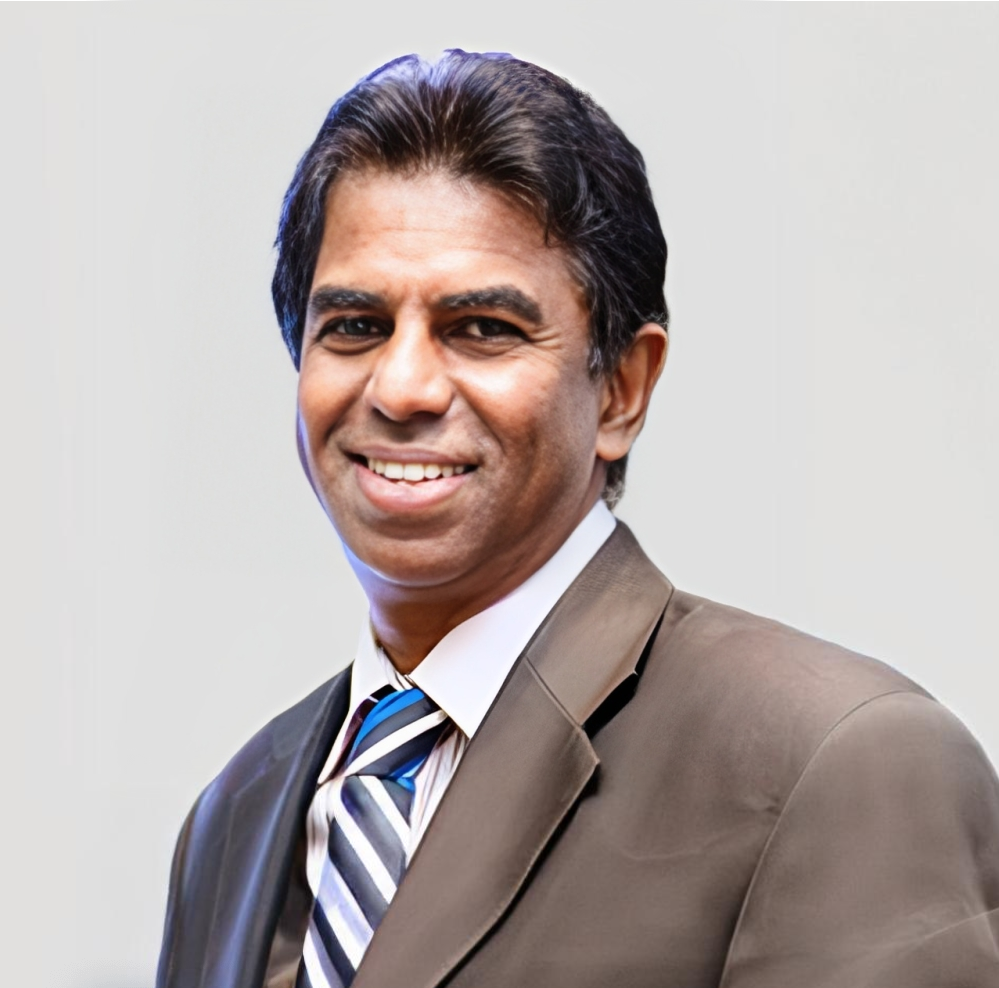
\includegraphics[width=0.3\textwidth]{Images/Keynote1.png}
% 	\end{wrapfigure}
% 	\vspace{2em} % Adjust vertical space as needed


\addmessage{Keynote Speaker}{Keynote1.png}

	
	I like to provide my warm congratulations to this very important International Research symposium on “Vocational Technology Education for a Sustainable Greener Economy”. marking another significant occasion in the journey of the University of Vocational Technology. Multi-disciplinary research and collaborations are essential to achieve a greener economy leading towards net zero and UN Sustainable development goals. This symposium provides that platform with 5 sub-themes covering several disciplines.
 
With your continued support and dedication, I am confident that the University of Vocational Technology will continue to lead the way in fostering sustainability and green practices in the industry, thus contributing to an eco-friendly future for Sri Lanka,
The achievements reached thus far would not have been possible without the dedication and hard work of the organizing committee led by the Symposium Chair Ms. Madhavi Perera. I also would like to acknowledge Ms Samantha Manawadu, who has won many Green Building Council awards,  for making my presence possible.
	
	\vspace{1cm}
	\noindent
	Prof. Priyan Mendis \\
Professor University of Melbourne, Australia \\
Founder Chairman,\\
Green Building Council of Sri Lanka
	
	\newpage
	
\thispagestyle{fancy}
	
% 	\vspace{-2em} % Adjust vertical space as needed
% 	\begin{center}



% \addcontentsline{toc}{subsection}{Message of the Guest of Honour}    
% \subsection*{\textsc{Message of the Guest of Honour}}
% 	\end{center}

   
    
%     \begin{wrapfigure}{l}{0.3\textwidth}
% 		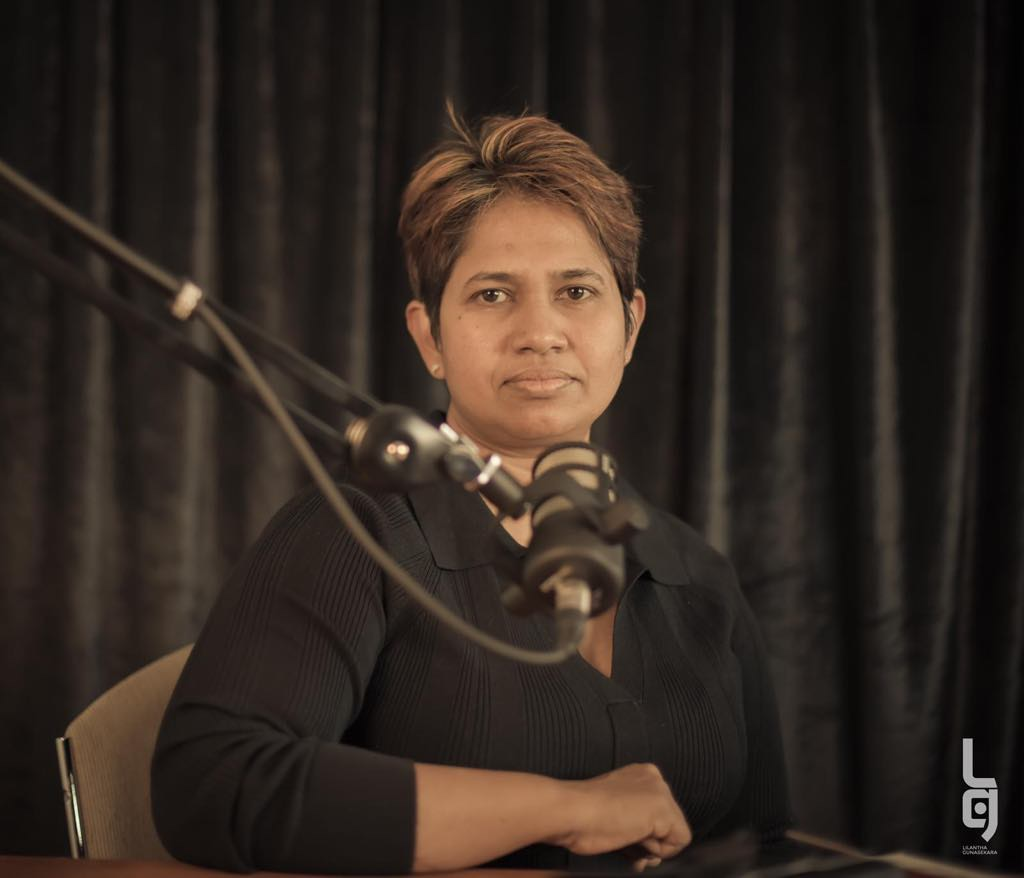
\includegraphics[width=0.3\textwidth]{Images/Guest1.jpeg}
% 	\end{wrapfigure}
% 	\vspace{2em} % Adjust vertical space as needed



\addmessage{Guest of Honour}{Guest2.jpeg}
	


It is an honor to contribute to the University of Vocational Technology Symposium 2024 as a guest speaker on the theme, “Empowering Dreams: Unlocking Higher Education Research Pathways for Vocational Excellence.”
Vocational education is a cornerstone of any nation’s economy, workforce development, and educational progress. By bridging the gap between industry needs and academic expertise, it equips individuals with skills that drive innovation and growth. Since its inception, the University of Vocational Technology has been a pioneer in this mission, nurturing talent and advancing vocational excellence in Sri Lanka.

Through its visionary free education system, Sri Lanka has the potential to achieve its aspirations by fostering research-driven solutions, enhancing global competitiveness, and shaping a resilient, skilled workforce. By investing in vocational education, we are not only empowering individuals but also driving the nation towards a future of sustainable development and economic prosperity.
The University of Vocational Technology stands as a beacon of hope and progress, demonstrating the transformative power of education. Its commitment to excellence and innovation has set a benchmark for vocational institutions worldwide. As we gather to discuss and share insights, let us remember the profound impact that vocational education has on our society. It is through these efforts that we can build a more inclusive and dynamic economy, where every individual has the opportunity to thrive.

Thank you for the privilege of sharing in this important conversation. Together, we can unlock the potential of dreams and pave the way for a brighter future. Let us continue to champion vocational education as a catalyst for national progress and global advancement.

\vspace{1cm}
	\noindent
    

Dr Nadeesha Chandrasena \\
Urban Innovator
	
	\newpage
	
\thispagestyle{fancy}
	
	\vspace{-2em} % Adjust vertical space as needed
% 	\begin{center}



% \addcontentsline{toc}{subsection}{Message of the Dean, Faculty of Education}    
% \subsection*{\textsc{Message of the Dean, Faculty of Education}}
% 	\end{center}

   
    
%     \begin{wrapfigure}{l}{0.3\textwidth}
% 		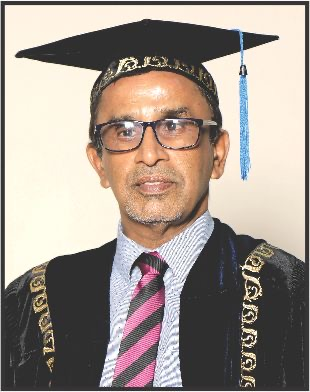
\includegraphics[width=0.3\textwidth]{Images/DeanFE.jpeg}
% 	\end{wrapfigure}
% 	\vspace{2em} % Adjust vertical space as needed


\addmessage{Dean, Faculty of Education}{DeanFE.jpeg}

	
	
	
	
	It is a great pleasure to issue this message on the occasion of the International Research Symposium (IRS), 2024 of the University of Vocational Technology. The Symposium is an annual event in the academic calendar of the University and has been a great success in the last several years.
    
The University has continued to promote conducive environment for increased generation of quality research while enabling mentorship of early researchers through research methodology and data analysis capacity development. We believe that dissemination of knowledge and providing    exposure to staff and students to engage in research is a part of our responsibility. It is a great opportunity for them to improve their analytical skills and interact with a wider community.

This annual symposium will provide an excellent platform for students and faculty members of the University, other public and private universities and research institutions to show-case their research productivity and promise for the future new knowledge generation.

Finally, I would like to thank the organizing committee and others who have worked hard to contribute to the success of this symposium.
 


	\vspace{1cm}
	\noindent
	Dr.Sunil Kularatne\\
Dean\\
Faculty of Education
	\newpage
	
\thispagestyle{fancy}
	
% 	\vspace{-2em} % Adjust vertical space as needed
% 	\begin{center}



% \addcontentsline{toc}{subsection}{Message of the Dean, Faculty of Engineering Technology}    
% \subsection*{\textsc{Message of the Dean, Faculty of Engineering Technology}}
% 	\end{center}

   
    
%     \begin{wrapfigure}{l}{0.3\textwidth}
% 		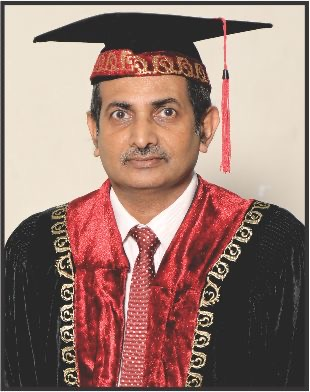
\includegraphics[width=0.3\textwidth]{Images/DeanFET.jpeg}
% 	\end{wrapfigure}
% 	\vspace{2em} % Adjust vertical space as needed


\addmessage{Dean, Faculty of Engineering Technology}{DeanFET.jpeg}

		It is a great pleasure to have an opportunity to convey my best wishes to the 8th International Research Symposium (IRS-2024) of the University of Vocational Technology. I want to express how proud I am of the hard work you have all put into your research works. This event highlights the diversity of ideas and perspectives that enrich our community, allowing us to learn from one another and discover new approaches to the important challenges we face today.
        
This symposium is not just about presenting your work; it is also a fantastic opportunity to share ideas and engage in meaningful conversations. Connecting with fellow researchers and industry professionals can spark innovative ideas and lead to valuable collaborations. Remember, the insights you gain from each other can inspire new directions in your research and open doors to exciting possibilities.

As you present your research, keep in mind that the journey of discovery is just as important as the results. Embrace the spirit of exploration and creativity that drives your work. Consider how your findings can contribute to broader conversations in your field and make a positive impact in the community. I am excited to hear about the remarkable work you have accomplished and to see the engaging discussions that will take place throughout the symposium. Together, we can celebrate our achievements and inspire one another to reach even greater heights.

	\vspace{1cm}
	\noindent
	Dr. Jayalal Wettasinghe\\
Dean\\
Faculty of Engineering Technology
	
	\newpage
\thispagestyle{fancy}
	
	\vspace{-2em} % Adjust vertical space as needed
	\begin{center}



\addcontentsline{toc}{subsection}{Message of the Dean, Faculty of Information Technology}    
\subsection*{\textsc{Message of the Dean, Faculty of Information Technology}}
	\end{center}

   
    
    \begin{wrapfigure}{l}{0.3\textwidth}
		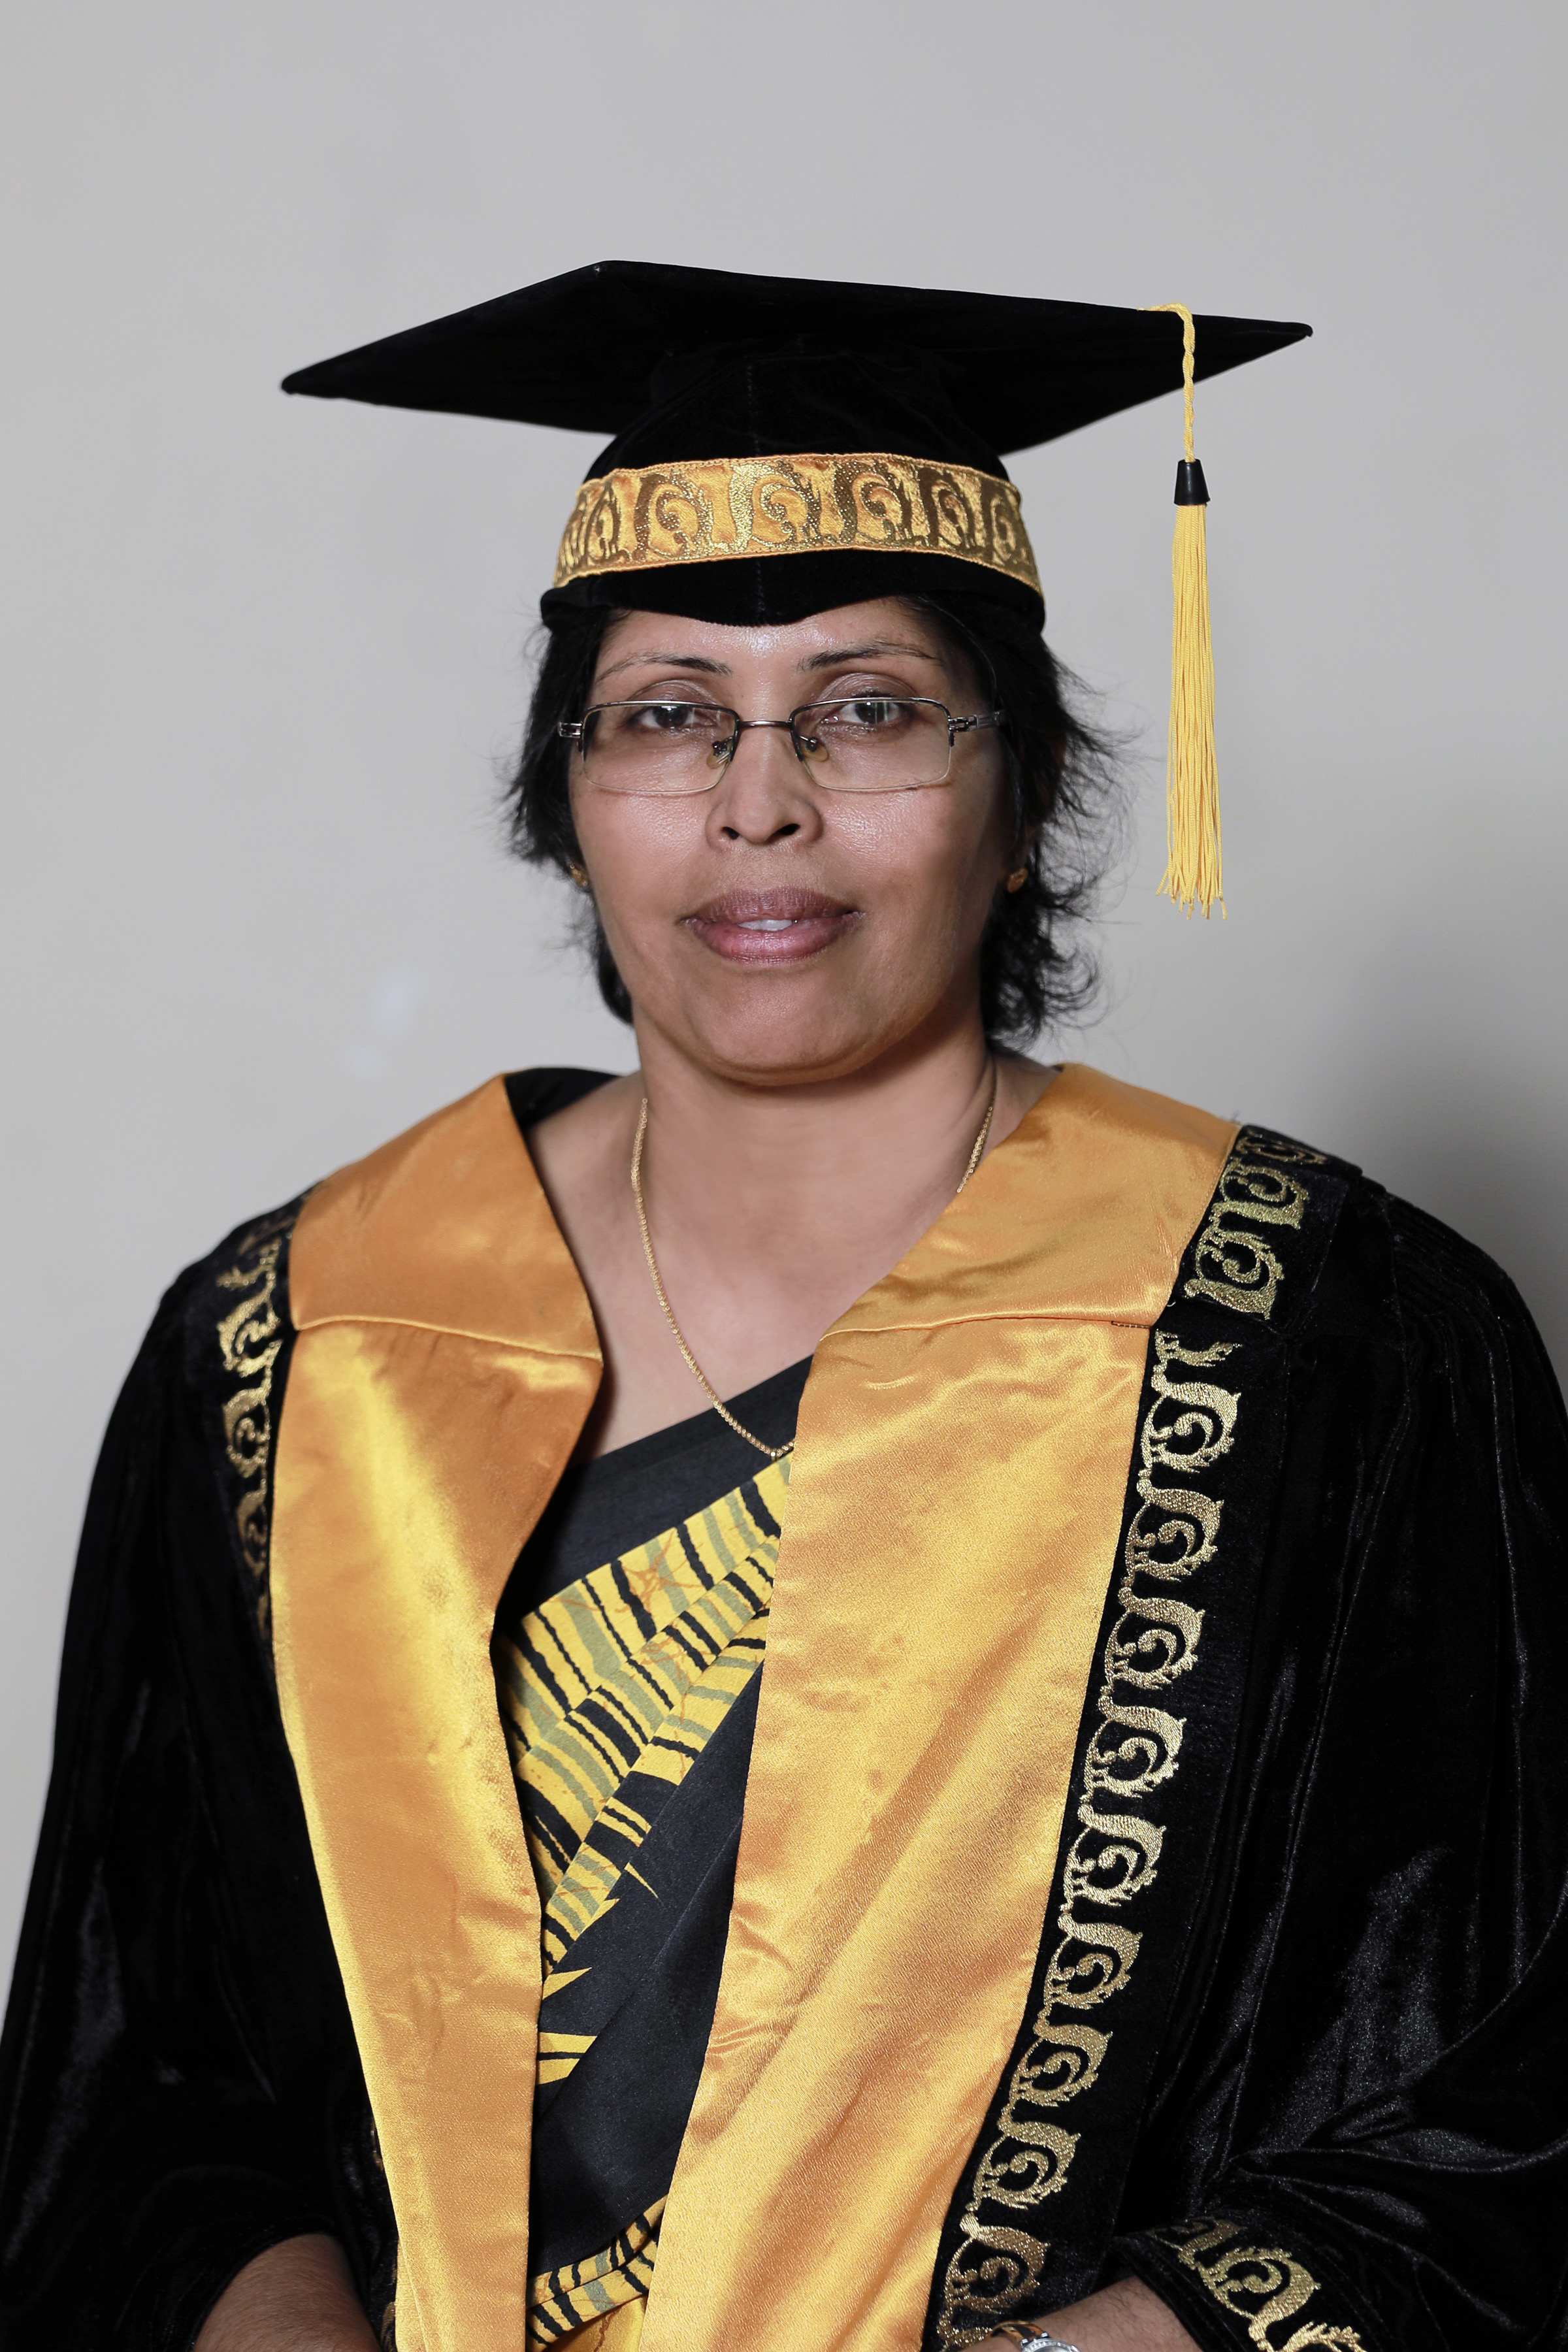
\includegraphics[width=0.3\textwidth]{Images/DeanICT.jpeg}
	\end{wrapfigure}
	\vspace{2em} % Adjust vertical space as needed




	
	\noindent	Dear Participants,\\
	
	\noindent
	Welcome to the International Research Symposium 2023. We are delighted to have you here and look forward to an engaging and productive event. 
	
	Welcome to the International Research Symposium 2023. We are delighted to have you here and look forward to an engaging and productive event. Welcome to the International Research Symposium 2023. We are delighted to have you here and look forward to an engaging and productive event. Welcome to the International Research Symposium 2023. We are delighted to have you here and look forward to an engaging and productive event. Welcome to the International Research Symposium 2023. We are delighted to have you here and look forward to an engaging and productive event. Welcome to the International Research Symposium 2023. We are delighted to have you here and look forward to an engaging and productive event. Welcome to the International Research Symposium 2023. We are delighted to have you here and look forward to an engaging and productive event. 
	
	
	Welcome to the International Research Symposium 2023. We are delighted to have you here and look forward to an engaging and productive event. Welcome to the International Research Symposium 2023. We are delighted to have you here and look forward to an engaging and productive event. Welcome to the International Research Symposium 2023. We are delighted to have you here and look forward to an engaging and productive event. Welcome to the International Research Symposium 2023. We are delighted to have you here and look forward to an engaging and productive event. Welcome to the International Research Symposium 2023. We are delighted to have you here and look forward to an engaging and productive event. Welcome to the International Research Symposium 2023. We are delighted to have you here and look forward to an engaging and productive event. 
	
	\vspace{1cm}
	\noindent
	Sincerely,\\
	Chairman's Name
	
	\newpage
	
\thispagestyle{fancy}
	
	\vspace{-2em} % Adjust vertical space as needed
	\begin{center}



\addcontentsline{toc}{subsection}{Message of the Dean, Faculty of Industrial Technology}    
\subsection*{\textsc{Message of the Dean, Faculty of Industrial Technology}}
	\end{center}

   
    
    \begin{wrapfigure}{l}{0.3\textwidth}
		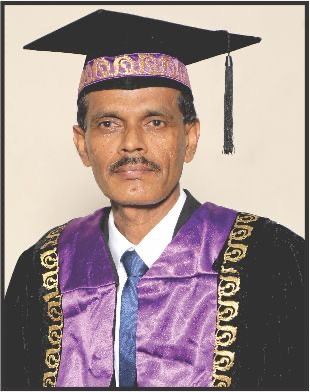
\includegraphics[width=0.3\textwidth]{Images/DeanFIT.jpeg}
	\end{wrapfigure}
	\vspace{2em} % Adjust vertical space as needed




	
	Greetings from the 2024 International Research Symposium, an exciting platform for innovation, learning, and collaboration. On behalf of the Faculty of Industrial Technology, it is my great honor to address all of you as we gather to explore groundbreaking research and insights across diverse fields.
Our faculty consists of four dynamic departments: Film and Television Production Technology, Agriculture and Food Technology, Industrial Management, and Quantity Surveying. These departments drive our mission of nurturing future leaders equipped with the knowledge, skills, and entrepreneurial spirit to meet the evolving needs of industries worldwide.

We provide six Bachelor of Technology degree programs that are uniquely tailored to meet industry standards: Media and Arts Production Technology, Film and Television Production Technology, Food Process Technology, Industrial Management, Hotel Management, and Quantity Surveying. In order to ensure that our graduates not only succeed in their chosen disciplines but also possess the abilities to innovate, adapt, and lead in the rapidly evolving technological landscape, our academic programs place a strong emphasis on techno-entrepreneurship. At the Faculty of Industrial Technology, we are committed to fostering a research and innovation culture among our students and faculty members. This symposium reflects our ongoing efforts to promote academic excellence, encourage knowledge sharing, and inspire new solutions to the challenges facing industries today.

I urge everyone to think creatively and courageously as we have meaningful conversations and share ideas. Let's work together to influence industry, science, and technology in order to create a sustainable and prosperous future.

	
	\vspace{1cm}
	Dr. Kamal Edirisinghe\\
Dean\\
Faculty of Industrial Technology
%\thispagestyle{fancy}
	
% 	\vspace{-2em} % Adjust vertical space as needed
% 	\begin{center}



% \addcontentsline{toc}{subsection}{Message of the Symposium Chair}    
% \subsection*{\textsc{Message of the Symposium Chair}}
% 	\end{center}

   
    
%     \begin{wrapfigure}{l}{0.3\textwidth}
% 		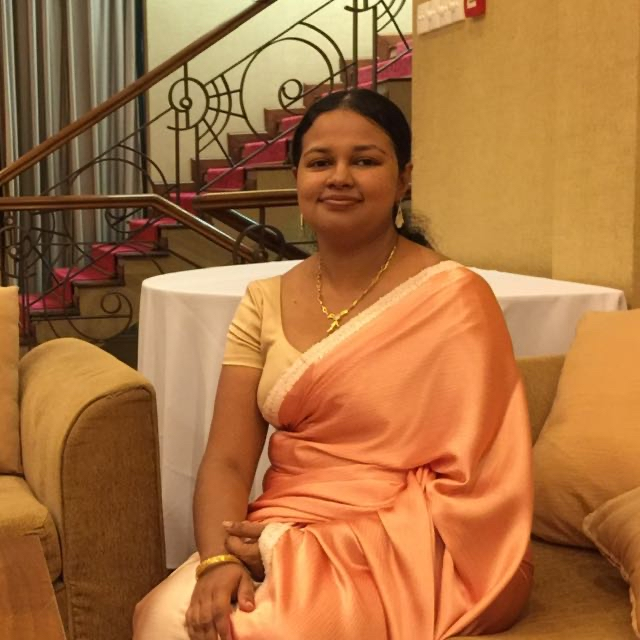
\includegraphics[width=0.3\textwidth]{Images/chair.jpeg}
% 	\end{wrapfigure}
% 	\vspace{2em} % Adjust vertical space as needed


\addmessage{Symposium Chair}{chair.jpeg}

	
As the Symposium Chair of IRS 2024 it is  an honour for me to welcome all of you to IRS 2024. This year, University of Vocational technology is very proudly hosting IRS 2024  under theme “Vocational Technology Education for Sustainable Greener Economy" . It is the 8\textsuperscript{th} research symposium organized by the university  and  IRS has become a tradition in the university and it has fostered a research culture in the university and it has been beneficial for  all of us to advance in our research careers.

This year’s theme marks an important responsibility that has being entrusted to University of Vocational Technology as the only university catering to TVET sector in the country.  With the whole world, Sri Lanka too is planning to steer our economy towards sustainable development and green economy. During this journey our  country will  need an empowered skillful work force who  can adopt to dynamic challenging situations and  TVET sector will be entrusted with building this  workforce.  We believe IRS 2024 will be an ideal platform to present research outputs and disseminate new knowledge that can empower the TVET sector professionals  to thrive and meet these new challenging goals.

The feedback we received for this symposium was beyond our expectations and we received a large number of research papers in  various fields that are aligning with our five tracks. All the papers were evaluated through blind review process by at least two subject experts and the feedback was given to the authors to improve the quality of their research work and the papers meeting the expected academic and research standards were selected for the presentations. On behalf of the program committee , I extend my heartiest gratitude towards all the reviewers who dedicated their valuable time and provided us the feedback required to maintain the academic standards of the symposium.  


Congratulations to all the authors on your achievement and we are looking forward to a productive day of disseminating knowledge and insightful discussions. I am confident that the proceedings of  IRS 2024 will inspire all of us to explore new research paths and conduct prominent research work in our respective fields.



% As the Symposium Chair of IRS 2024, it is an honour to welcome you all. This year, the University of Vocational Technology proudly hosts IRS 2024 under the theme “Vocational Technology Education for Sustainable Greener Economy.” This 8th research symposium has become a tradition, fostering a research culture and benefiting our careers.

% This year’s theme highlights the responsibility of the University of Vocational Technology as the only university catering to the TVET sector in the country. Sri Lanka is steering towards sustainable development and a green economy, requiring a skilled workforce. TVET will build this workforce. IRS 2024 is an ideal platform to present research in sustainable TVET, innovation, entrepreneurship, and sustainable practices in industrial, digital, and engineering technologies.

% We received a large number of research papers, evaluated through a blind review process by subject experts. Selected papers met academic and research standards. I extend gratitude to all reviewers for their valuable feedback.

% I thank the Vice Chancellor for guidance and mentorship, and all staff members for their dedication. Congratulations to all authors. We look forward to a productive day of knowledge dissemination and discussions. I am confident IRS 2024 will inspire new research paths and prominent work in our fields.

	% \vspace{1cm}
	% \noindent
    
Ms. P.M. Perera \\
Symposium Chair - International Research Symposium 2024 - UOVT


	\newpage
	








\setcounter{page}{1}
\pagenumbering{arabic}


% \AddToShipoutPicture{%
%     \begin{tikzpicture}[remember picture,overlay]
%         \nodeanchor=north east,inner sep=0pt,yshift=1cm,xshift=1cm at (current page text area.north east){\hyperlink{page.iii}
%             {\transparent{0.6} {\includegraphics[width=0.3cm]{home.jpeg}}}};
%     \end{tikzpicture}
% }




%% \addpaper{paper title} {Authors' Names} {PDF path}
%   		 
%   		 

\sessiontitle{Track 1}{Educational Strategies for Sustainable TVET}


\addpaper
	{Effectiveness of the Mind Mapping Technique in Essay Writing: A Case Study of Grade 11 ESL Learners}
	 {S.G.M.D.S. Senavirathne and D.D.D. Suraweera} 
	 {Papers/Track1/13.pdf}
    {13} 


  \addpaper
{An analysis of pronunciation teaching inclusion into Sri Lankan English textbooks from grade three to G. C. E. (A/L)}
 {R. M. Azver and A. A. Gunawardana} 
 {Papers/Track1/18.pdf}
   {18} 

  \addpaper
{Needs Analysis of English for Academic Purposes for ELT Undergraduates}
 {V.T.D.M. Kulathilaka and J. A. M. Buddhima Karunarathna} 
 {Papers/Track1/29.pdf}
   {29} 
 


\addpaper
{a case study of academic, social and family history and behavioural situation of below average level student readers with spelling and word recognition challenges}
{S.S.S. De Silva}
{Papers/Track1/46.pdf}
{46}


%    \addpaper
% {an exploratory case study on ESL teachers' perceptions and practices in fostering learner autonomy to enhance the english language competency of ESL learners.}
%  {Chathurangi U Karunasena} 
%  {Papers/Track1/51.pdf}
%    {51} 


   \addpaper
{enhancing learners’ intrinsic interest in english language learning through oral acknowledgement: acknowledging students’ minimum effort for maximum impact}
 {K.G.H.S. Chandrasekara and C.L. Amarasekara} 
 {Papers/Track1/57.pdf}
   {57} 


\addpaper
{Indices to Consider for Further Development of Degree Programs: Case Study-University of Vocational Technology, Sri Lanka}
{U. Sivachelvy, S.R. Muditha Seneviratne, P. Uruthiran and N.B.W.I. Udeshika}
{Papers/Track1/74.pdf}
{74}


\addpaper
{Challenges Faced by Students in Learning English as a Second Language for G.C.E. O/L Examination in Puttlam South Education Division}
{W. R. A. D. Lakshani and K. T. P. C. Somarathna}
{Papers/Track1/80.pdf}
{80}


    \addpaper
{the impact of university lecturers' attitudes on
undergraduate’s academic outcomes: A
comparative analysis across europe, asia, and sri
lanka}
 {D.V. Durga Sajeevani, Malkanthi Thenabadu and M. H. Methmini Tharanga} 
 {Papers/Track1/150.pdf}
   {150} 


\addpaper
{the role of powerpoint presentations in online education; A case study based on university of vocational technology, sri lanka}
{A. S. U. Dharmadasa and K. D. S. S. Karunasinghe}
{Papers/Track1/02.pdf}
{02}


\addpaper
{factors affecting to the selection of courses in university colleges, sri lanka}
{W.A.M. Hansika}
{Papers/Track1/3.pdf}
{03}




   \addpaper
{ESL Teacher Competence in Integrating Technology with ESL Instruction: A Comparative Study between Government and Private Sector In-Service ESL Student-Teachers}
 {R.T.V. Madushani and A.A. Gunawardana} 
 {Papers/Track1/12.pdf}
   {12} 


\addpaper
{Perceptions of instructors on the use of EGP and ESP in teaching english: A study carried out in technical and vocational education and training institution}
{V. S. Dileka Thennakoon and Dilini Ranasuriya}
{Papers/Track1/44.pdf}
{44}


\addpaper
{Sustainable TVET: The Descriptive Study on the Barriers to Developing the English Language Among TVET Skill Learners}
{U. P. N. S. Gunathunga and Dilini Ranasuriya}
{Papers/Track1/94.pdf}
{94}


   \addpaper
{Usage of ICT Tools in the Teaching and Learning Process in the Technical and Vocational Sector: Technology Acceptance Model (TAM) Approach}
 {Mahalingam Ramanan} 
 {Papers/Track1/96.pdf}
   {96} 


\addpaper
{Exploring the influence of Gender in the Adoption of Digital Platforms for Entrepreneurship: A Study Among Higher National Diploma Students in Colombo, Sri Lanka}
{H.A. Seneviratne}
{Papers/Track1/113.pdf}
{113}

\addpaper
{Enhancement of Career Guidance for Vocational Training Recipients of Vocational Training Authority of Sri Lanka}
{Yamuna Manathunge , Prasanna Illankoon and E. A. D. Senarathne}
{Papers/Track1/136.pdf}
{136}


\addpaper
{Gamification as an Innovative Teaching Methodology to Engage and Motivate Learners for Sustainable Technical and Vocational Education and Training}
{Janaka Jayalath}
{Papers/Track1/148.pdf}
{148}



\addpaper
{Exploring lecturers' Perceptions on Mobile Assisted Language Learning in ESL Classroom: A case study}
{K. G. I. Madumalika and K. T. P. C. Somarathna}
{Papers/Track1/75.pdf}
{75}


\sessiontitle{Technical Session 2}{Engineering Technology for Green Economy} 




   \addpaper
    	{a case study on cost-benefit analysis to assess the profitability of installing solar panels at the irrigation department head office in colombo}
   		 {S. S. Yamasinghe and U. Sivachelvy} 
   		 {Papers/Track2/62.pdf}
        {62} 

        
   %      \addpaper
   %  	{Factors Influencing Intention to Purchase Residential Solar Panel Systems in Sri Lanka}
   % 		 {G Thilak Kumar} 
   % 		 {Papers/Track2/98.pdf}
   %      {98} 

        
   %      \addpaper
   %  	{development of an automate solar panel cleaning system}
   % 		 {S.P.A.R.S Jayathilaka} 
   % 		 {Papers/Track2/106.pdf}
   %      {106} 

        
   %      \addpaper
   %  	{Green Energy and Social Equity: Addressing Disparities in Access and Benefits}
   % 		 {Tashni P Herath} 
   % 		 {Papers/Track2/116.pdf}
   %      {116} 

        
   %      \addpaper
   %  	{Electro-Magnetic Interference Filter For Ultrasound Scanner}
   % 		 {Jayaweera K Kanthi} 
   % 		 {Papers/Track2/82.pdf}
   %      {82} 

        
   %      \addpaper
   %  	{Design and Implementation of a Power Monitoring System for Industrial Applications}
   % 		 {Ashan Nimsara Yapa and Sudeepa M Herath} 
   % 		 {Papers/Track2/11.pdf}
   %      {11} 

        
   %      \addpaper
   %  	{Assessing the feasibility and potential of Vertical Axis Wind Turbines (VAWTs) as a sustainable energy source for remote university settings}
   % 		 {Dinithi M Warakagoda} 
   % 		 {Papers/Track2/14.pdf}
   %      {14} 

        
   %      \addpaper
   %  	{Advancements and Impacts of Combine Harvesters in Paddy Cultivation in Northern Sri Lanka: A Comprehensive Review}
   % 		 {Murugaiyah Priyatharsini} 
   % 		 {Papers/Track2/65.pdf}
   %      {65} 

        
   %      \addpaper
   %  	{A Review on Existing Tricycle Suspension Systems}
   % 		 {Nilushika Sudarshani Menike} 
   % 		 {Papers/Track2/67.pdf}
   %      {67} 

        
        \addpaper
    	{design of automated oil-water separator systems to reduce environmental effects in associated industries}
   		 {H.I. Pushpakumara and Sasiri Gamage} 
   		 {Papers/Track2/87.pdf}
        {87} 

        
        \addpaper
    	{Sugarcane Bagasse Ash as a Partial Substitute for Fine Aggregate in Cement-Based Products}
   		 {T. M. S. Madhushika, K. G. Alahapperuma and D. D. D. Suraweera} 
   		 {Papers/Track2/90.pdf}
        {90} 

        
     %    \addpaper
    	% {A Review on Chassis Systems of Tricycles}
   		%  {Tharindu Deshan Delpachithra} 
   		%  {Papers/Track2/71.pdf}
     %    {71} 

        
     %    \addpaper
    	% {Investigation of burned timber ash as a partial substitute of cement in soil-cement mix as a backfilling material in small-scale building construction}
   		%  {Shankani Gunarathna} 
   		%  {Papers/Track2/160.pdf}
     %    {160} 

        
        \addpaper
    	{A Comprehensive Investigation into the Applications, Barriers and Future Directions of Drone Technology Sri Lanka Construction Management}
   		 {K. Vaitheki} 
   		 {Papers/Track2/07.pdf}
        {7} 

        
     %    \addpaper
    	% {Investigating the Potential of 4D Printing for Sustainable Solutions in Civil Engineering: A Systematic Review}
   		%  {Kamalaseelan Kajeenthan and Pirabakaran Kavippriyan} 
   		%  {Papers/Track2/8.pdf}
     %    {8} 

     
        \addpaper
    	{determination of applicability clay from the abandoned tile factory yatiyana, matara, sri lanka for a wall tile design}
   	   {D.S. Abeygunawardana and T.D. Denagama} 
   		 {Papers/Track2/19.pdf}
        {19} 

        
        \addpaper
    	{A Comprehensive Analysis of the Role of Digital Twin Technology in the Construction Industry}
   		 {K. Vaitheki and J. Dhanuj} 
   		 {Papers/Track2/72.pdf}
        {72} 

        
     %    \addpaper
    	% {Case Studies of Soft Active Materials for Engineering Applications}
   		%  {Mapa Mudhiyanselage Lahiru Pemachandra} 
   		%  {Papers/Track2/93.pdf}
     %    {93} 

        
     %    \addpaper
    	% {failures in project completion}
   		%  {Hashan Tharindu Fonseka} 
   		%  {Papers/Track2/2.pdf}
     %    {130} 

        
        \addpaper
    	{Minimizing Variation Orders in the Construction of Married Quarters for Special Task Force, Sri Lanka: A Case Study}
   		 {E.S.N Nadeeshani} 
   		 {Papers/Track2/138.pdf}
        {138} 

        
     %    \addpaper
    	% {Assessing the impact of utility cuts practices on the service life of flexible pavement in Sri Lanka}
   		%  {Imalka Subhashini Jayasundara} 
   		%  {Papers/Track2/139.pdf}
     %    {139} 

        
     %    \addpaper
    	% {Delay in Progress due to Late Payment; the Case of Historic Rajawasala Restoration Project in Kandy}
   		%  {Vindya H Epanage (S.E.V.H Epanage )} 
   		%  {Papers/Track2/142.pdf}
     %    {142} 

        
        \addpaper
    	{Evaluation of Bonding Strength and Cost Effectiveness of a Substitute Internal Plastering Mix}
   		 {J. A. D. P. Anjana Jayasuriya and Kasun Nandapala} 
   		 {Papers/Track2/152.pdf}
        {152} 

        
     %    \addpaper
    	% {Experimental Investigation to find out solution for Pepper joint waterproofing at ITC Project}
   		%  {Thanuka R Gunathilake and Kasun Nandapala} 
   		%  {Papers/Track2/39.pdf}
     %    {39} 

        
     %    \addpaper
    	% {causes and impacts of variation orders in the grand tower residencies apartment project: a case study in colombo, sri lanka}
   		%  {Mohamed Rikas and Mohamed Rikas} 
   		%  {Papers/Track2/102.pdf}
     %    {102} 

        
         \addpaper
    	{Use of Coconut Coir as a Reinforcing Material in Clay Bricks}
   		 {K. G. Alahapperuma, E. R. Madhushanka, G. T. Madhushani and R. G. P. C.Rajamanthri} 
   		 {Papers/Track2/56.pdf}
        {56} 

        
     %     \addpaper
    	% {Cost Effective Wireless Guestroom Control System}
   		%  {Madhavi Perera} 
   		%  {Papers/Track2/159.pdf}
     %    {159} 

        
         \addpaper
    	{Impact of Building Services on Customer Satisfaction in Sri Lankan Hotels}
   		 {N.S. Karunasinghe} 
   		 {Papers/Track2/83.pdf}
        {83} 

        
     %     \addpaper
    	% {Air Quality of Air-Conditioned and non-air-conditioned Buses}
   		%  {Pathiranage pubudu} 
   		%  {Papers/Track2/121.pdf}
     %    {121} 

        
     %     \addpaper
    	% {Low Cost Solar Powered Daylight Tube for Residential Buildings in Sri Lanka}
   		%  {Madhavi Perera} 
   		%  {Papers/Track2/158.pdf}
     %    {158} 

        
     %     \addpaper
    	% {Evaluating the Thermal Insulation Properties of Mushroom Production Waste in Building Applications}
   		%  {Harshani R.M.M. Upamalika , Sanjaya Kumara , Thiruvakaran Luckshanth and Kasun Nandapala } 
   		%  {Papers/Track2/109.pdf}
     %    {109} 

        
     %     \addpaper
    	% {Innovative Strategies for Minimizing Material Wastage on Electrical Service Construction. A Case Study Analysis for Hotel Building Project in Sri Lanka}
   		%  {Madushani Kaushalya } 
   		%  {Papers/Track2/111.pdf}
     %    {111} 

        
     %     \addpaper
    	% {Identification of best plant combinations in increasing the thermal conductivity of vertical green systems under tropical climatic conditions}
   		%  {Samantha Manawadu} 
   		%  {Papers/Track2/161.pdf}
     %    {161} 

        
     %     \addpaper
    	% {Analysis of Frequent Electrical Breakdowns in Mawanella: Causes, Impacts, and Mitigation Strategies}
   		%  {Prasad Dissanayake} 
   		%  {Papers/Track2/157.pdf}
     %    {157} 

        
         \addpaper
    	{Development of a Non-Lethal Wildlife Deterrent System: Addressing Human-Wildlife Conflict with Asian Palm Civets in Agricultural and Residential Areas}
   		 {M.H.M Hadhil and S.V.R Gamage} 
   		 {Papers/Track2/79.pdf}
        {79} 

        
     %     \addpaper
    	% {Image-Based Quality Inspection in Metal Roofing Sheets Products Using Image Processing}
   		%  {Sondarangallage D.A Sanjeewa} 
   		%  {Papers/Track2/95.pdf}
     %    {95} 

        
     %     \addpaper
    	% {Automation of Traditional Agriculture: Robot Harvesting with Challenges}
   		%  {Duminda S.B. Ratnayake} 
   		%  {Papers/Track2/99.pdf}
     %    {99} 

        
     %    \addpaper
    	% {advanced wheel chair control system rasberry pi-3-based joystick analog and voice control}
   		%  {Dilshan T Ganegoda} 
   		%  {Papers/Track2/108.pdf}
     %    {108} 

        
     %    \addpaper
    	% {Design and Implementation of Smart Shock Absorber Integrated with GPS-Based Road Condition Analysis}
   		%  {Barathy M Aklakurajah} 
   		%  {Papers/Track2/112.pdf}
     %    {112} 

        
     %    \addpaper
    	% {Design a Full-Body Covered Safety Airbag System for Motorcyclists}
   		%  {Barathy M Aklakurajah} 
   		%  {Papers/Track2/114.pdf}
     %    {114} 

        
     %    \addpaper
    	% {Error Detection of The Tower Parts in Tower Fabrication Industry by Image Processing}
   		%  {Sondarangallage D.A Sanjeewa} 
   		%  {Papers/Track2/133.pdf}
     %    {133} 
     
         \addpaper
    	{demolition waste management of CIDA-registered construction companies in jaffna district and possible improvement strategies}
   		 {K. Thifya and T.D. Denagama} 
   		 {Papers/Track2/30.pdf}
        {30} 

        \addpaper
    	{an assessment of water quality related issues in polgolla reservoir, sri lanka}
   		 {A.P.G.G.C. Bogahawaththa and T.D. Denagama} 
   		 {Papers/Track2/20.pdf}
        {20}

        \addpaper
    	{Determination of Effectiveness of Domestic Sewerage System in High Water Table Area at Sathsevana Childerns' Home in Mirigama Sri Lanka}
   		 {S.D.G.M. Sirimanna and T.D. Denagama} 
   		 {Papers/Track2/21.pdf}
        {21}

\sessiontitle{Track 3}{Digital Technologies and Creative Industries} 



  \addpaper
    	{Analysis the Influence Factors of the Indoor Path Loss Calculation}
   		 {L. P. S. S. Dissanayake, D. M. L. M. Dissanayake and H. P. A. I. Pathirana} 
   		 {Papers/Track3/54.pdf}
        {54}


    \addpaper
    	{Developing a Specialized Job Board for NVQ Certificate Holders in Sri Lanka}
   		 {J.K.B.E. Sanadruwani, S.S. Wijayarathna and A. Seneviratne} 
   		 {Papers/Track3/103.pdf}
        {103}

    
 \addpaper
    	{Next-Generation School Bus Tracking: A Mobile-Centric Approach for Real-Time Monitoring}
   		 {H. P. A. I. Pathirana, R. M. S. Ruvishan, S. M. S. S. M. Seelawansha and D. M. D. S. Dissanayake} 
   		 {Papers/Track3/120.pdf}
        {120}




   \addpaper
    	{An Enhancing Public Transportation in Sri Lanka Through Real-Time Tracking and Booking System}
   		 {K. P. V. N. Pathirage, A. I. Chathurangi, D. M. H. Madushani and P. Uruthiran} 
   		 {Papers/Track3/16.pdf}
        {16}

  
  \addpaper
    	{native tamil news article summarization}
   		 {Satheeskumar Y. and Chandana G.} 
   		 {Papers/Track3/05.pdf}
        {05}

  \addpaper
    	{strategies used in film marketing, case studies in hollywood film industry}
   		 {Nipuni Shehani Dompage and Nalin Galkanda Arachchi} 
   		 {Papers/Track3/135.pdf}
        {135}


%%%%%%%%%%%%%%% 37 %%%%%%%%%%%%%%%%%%%%%%%%
      \addpaper
    	{design and development of a database-driven application for sinhala etymological analysis}
   		 {K.P.D.S.L. Kodagoda and H.G.C.K. Hulangamuwa} 
   		 {Papers/Track3/28.pdf}
        {28}



    \addpaper
    	{Virtual Fitting Room System (FIT-ME)}
   		 {N.B.R.A. Apeksha, H.K.S. Malsha, R.A.R.D. Ranathunga and T.K. Malwatta} 
   		 {Papers/Track3/40.pdf}
        {40}

    \addpaper
    	{Development and Evaluation of an Automated Student Attendance Tracking System Using Facial Recognition Technology}
   		 {D. A. N. T. Perera , T. K. Malwatta , P. H. S. S. Wijerathne and L. S. M. N. D. Senanayaka} 
   		 {Papers/Track3/48.pdf}
        {48}


        


        
    % \addpaper
    % 	{Low Cost IoT-Based Home Remote Monitoring and Controlling System}
   	% 	 {Rukshanth Marudhapulle} 
   	% 	 {Papers/Track3/85.pdf}
    %     {85}

   

   

   


  
  

\sessiontitle{Track 4}{Innovation and Entrepreneurship for Economic Resilience}




\addpaper
{Generative AI-Powered Organizational Learning Cultures in Sri Lanka and Employees' Perceptions}
{D.L.N.P. Amarawickrama and U. Sivachelvy}
{Papers/Track4/26.pdf}
{26}

\addpaper
{Optimizing Inventory Through ABC-FSN Analysis}
{G. Wickramasinghe, Jayalal Wettasinghe and Kasun Lankapura}
{Papers/Track4/122.pdf}
{122}

   \addpaper
{Purchase Intention of Cloud Products: A Study of small and medium enterprise Customers in Leading Telecommunication Provider in Sri Lanka}
 {Rumesh Chathuranga Kumaradasa and Indika Priyantha Kaluarachchige } 
 {Papers/Track4/131.pdf}
   {131}

\addpaper
{Optimization of a Single Supplier Raw Materials Inventory System in a Fabric Manufacturing Plant}
{K. Lankapura and Jayalal Wettasinghe}
{Papers/Track4/134.pdf}
{134}

   \addpaper
{manufacturers' perception on establishing
refilling stations as a sustainable solution for
single-Use plastics: A study based on cleaning
liquid manufacturing industry}
 {K. G. S. S. Bandara, T. R. Vidanapathirane and H. M. A. P. P. Herath} 
 {Papers/Track4/91.pdf}
   {91}


   \addpaper
{Customer Churn of Fibre Retail Customers in Leading Telecommunication Service Provider in Sri Lanka}
 {S. H. Hettiarachchi and Indika P. Kaluarachchige} 
 {Papers/Track4/132.pdf}
   {132}


   
   

\addpaper
{An Effect of MAS Holdings in the Sri Lankan Garment Industry}
{Thiwanka Srinath K.M. and Sivachelvy U.}
{Papers/Track4/143.pdf}
{143}


\addpaper
{The Factors Influencing Tourists’ Satisfaction and Their Impacts on Destination Loyalty in Domestic Tourism in Sri Lanka}
{K. Shanmuganathan}
{Papers/Track4/35.pdf}
{35}



   \addpaper
{Review on skin depigmenting activity of common medicinal plants used in Sri Lankan traditional beauty remedies}
 {Gunarathna B.W.A.S. and Amali T.A.D.H.} 
 {Papers/Track4/38.pdf}
   {38}



   \addpaper
{Assessing the Entrepreneurial Intentions of Cosmetology Students in Sri Lankan University Colleges}
 {Nirmalan T.E., De Silva J.H.I.G. and Kiruththiga R.} 
 {Papers/Track4/43.pdf}
   {43}





\addpaper
{Review of Toxic Chemicals in Cosmetics}
{R.M.D.N. Bandara , J.H.I.G. De Silva and G.S. Prasanna}
{Papers/Track4/47.pdf}
{47}

\addpaper
{promoting sustainable nature tourism through visitor interpretative infrastructure as tourism educational tool in horton plains national park}
{U.A. Dhanusha Premarathna}
{Papers/Track4/92.pdf}
{92}

\addpaper
{Exploring the factors affecting on tourist satisfaction with ride-Sharing services in Sri Lanka (With Special Reference to Colombo District)}
{K.H. Pavithra and H.F.N.U. Fonseka}
{Papers/Track4/123.pdf}
{123}

\addpaper
{Challenge and Opportunities on Adopting Tourist Information Kiosks in Cultural Triangle Sri Lanka: Tourism Stakeholders' Perspective}
{H.P.M.S.K. Jayaweera and A.M.D.B. Nawarathne}
{Papers/Track4/129.pdf}
{129}

   \addpaper
{identifying the psychological aspects of digital nomads for tourism destination marketing in sri lanka}
 {A. K. D. T. Yohani, R. A. A. K. Ranaweera and M. M. G. K. Marasinghe} 
 {Papers/Track4/149.pdf}
   {149}


  \addpaper
{the local community involvement in developing
the Eco-Tourism: (special reference to meemure
tourism destination, sri lanka)}
 {K. A. D. I. Wickramarathne} 
 {Papers/Track4/155.pdf}
   {155}


\addpaper
{Preliminary Study on The Bragadi Thailaya of Thalpathe Piliyam for Darunaka}
{E.M.C.K. Ekanayake, S.P.A.U.M. Gunathilaka, K.A.I. Amarasinghe, S.D.N.M. Premathilaka, K.T.M. Jayasinghe, K.M.M. Sewwandi and P. Hewagamage}
{Papers/Track4/154.pdf}
{154}


   
   \addpaper
{Improving the Efficiency of the MTU Workshop at the Sri Lanka Naval Dockyard, Trincomalee}
 {A. N. L. Senarath, K. A. C. Sanjaya Kumara and Ravindra Koggalage} 
 {Papers/Track4/101.pdf}
   {101}



   \addpaper
{University working Students' Time Management and its Effect on Academic Success}
 {P.G.S.M. Chandrarathna and B.M.T.D. Jayasekara} 
 {Papers/Track4/137.pdf}
   {137}

   \addpaper
{challenges of tour guiding in sri lankan tourism
industry}
 {Gunasekara I.} 
 {Papers/Track4/147.pdf}
   {147}






\sessiontitle{Technical Session 5}{Sustainable Practices for Multifunctional Green Economy} 



   \addpaper
    	{A Review of Developed Lean Construction Frameworks in the Sri Lankan Context}
   		 {P.L. Perera, S. Kajewski and V. Coffey} 
   		 {Papers/Track5/01.pdf}
        {1} 

       \addpaper
    	{Towards the Development of a Specific Procurement Guideline for the Water Supply Sector in Sri Lanka}
   		 {Sisilaksha M.D.N and Seneviratne S.R.M.P} 
   		 {Papers/Track5/60.pdf}
        {60}

     %    \addpaper
    	% {Major Determinants of Site Level Labors Retention: The Case of Direct Skilled Labors of Sri Lanka}
   		%  {Muditha P Seneviratne and Ayanthika Subodhani S Gunathilaka} 
   		%  {Papers/Track5/63.pdf}
     %    {63}

     %    \addpaper
    	% {Construction projects performance attributes on Domestic Contractor’s Cost Controlling action of Sri Lankan construction industry}
   		%  {Damith Balasooriya, Muditha P Seneviratne and Thamara BMTD Jayasekara} 
   		%  {Papers/Track5/73.pdf}
     %    {73}

        \addpaper
    	{approaches to confront the sri lankan crisis as a successful local quantity surveyor}
   		 {Vijayaragunathan Srivishagan, Rasanthi Thalpage and B,T, Rifdhy} 
   		 {Papers/Track5/86.pdf}
        {86}

        \addpaper
    	{Mitigate the impacts of Project Delays on the Contractor’s Cash Flow: Case Study approach}
   		 {D. C. Wedikkara, C. Jayalath and S. R. M. P. Seneviratne} 
   		 {Papers/Track5/104.pdf}
        {104}

        \addpaper
    	{informal construction sector in sri lanka and its existing challenges: a way forward for formalizing}
   		 {R. Thalpage, V. Srivishagan and G.V. Mahesh Silva} 
   		 {Papers/Track5/49.pdf}
        {49}

        \addpaper
    	{Measures to overcome Project Complexity occurred over series of project revisions and overlapped variations transpired out of contractual scope: A case study approach}
   		 {M. M. Wijesirinarayana, Chandana Jayalath and S. R. Muditha Seneviratne} 
   		 {Papers/Track5/124.pdf}
        {124}

     %    \addpaper
    	% {Aptness of the CIDA Formula Method to Mitigate Construction Cost Uncertainties: Sri Lankan case study during economic recession}
   		%  {Hiroshani Yakupitiya Ruwanmali} 
   		%  {Papers/Track5/127.pdf}
     %    {127}

     %    \addpaper
    	% {Suggestions to Mitigating impacts of skilled labor shortage in Sri Lanka}
   		%  {Wathsala G.R Prasadini, Chandana Jayalath and Muditha P Seneviratne} 
   		%  {Papers/Track5/141.pdf}
     %    {141}

        \addpaper
    	{Mitigate the consequences on Contractor's profit by Variations at rural domestic residential construction: Case study: SME Construction Company of Sri Lanka}
   		 {B.M.H. Jayathilaka, Chandana Jayalath and S.R. Muditha Seneviratne} 
   		 {Papers/Track5/119.pdf}
        {119}

        \addpaper
    	{Determination of Nutritional and Functional Properties of Sri Lankan Traditional Fermented Rice}
   		 {D.M.M.M Premarathna, Chathuni Jayathilake and Malkanthi
         Thenabadu} 
   		 {Papers/Track5/04.pdf}
        {04}

        \addpaper
    	{qualitative detection of adulteration in non-Labeled chili and turmeric powders sold in the retail market in the matara city area}
   		 {K. M. N. K. Sewwandi , P. Varunitha, D. M. S. H. Dissanayake and
          J. M. C. M. Jayasekara} 
   		 {Papers/Track5/06.pdf}
        {6}

        \addpaper
    	{Development of Spreadable Creamed Coconut (Coconut Spread)}
   		 {Dasanayaka U.P.A.L. and Yogaprathish.V.} 
   		 {Papers/Track5/09.pdf}
        {9}

        \addpaper
    	{Consumer acceptability of Ceylon Date palm fruit incorporated alcoholic beverage}
   		 {I.P.D.P.D. Samanthilaka, W.A.C.H. Wijayathilaka and M.L.P. Thathsarani} 
   		 {Papers/Track5/31.pdf}
        {31}

     %    \addpaper
    	% {Development of a Monitoring System for Tracking and Analyzing Pre-packaged Fast Food Consumption}
   		%  {Rajitha Wasana Wedage} 
   		%  {Papers/Track5/37.pdf}
     %    {37}

        \addpaper
    	{Development and Characterization of a Coriander Leaf and Green Chili-Based Culinary Sauce}
   		 {P. Anusha, S. Danushan and P. Karthiha} 
   		 {Papers/Track5/41.pdf}
        {41}

        \addpaper
    	{Development and Evaluation of a Ready-to-Eat Ketogenic Bar: Formulation, Nutritional Composition, Sensory Properties}
   		 {Yasintha K.W, Pasan A.J.R. and P, Kumari E. M S.H} 
   		 {Papers/Track5/45.pdf}
        {45}

        \addpaper
    	{ingredient shelf-life management and safety: A case study of cinnamon hotels and resorts}
   		 {A.S.J. Chandimal, G.M. Somaratne, Y.D.M.D.C.Y. Bandara,
M.A. Samarasekara and N.M.A.I. Nikalansooriya} 
   		 {Papers/Track5/55.pdf}
        {55}

        \addpaper
    	{Development of Chocolate Alternative using Avocado Seed (Persea Americana) - A review}
   		 {A. D. M. P. Dissanayake and U.A.S.K. Edirisinghe} 
   		 {Papers/Track5/59.pdf}
        {59}



        \addpaper
    	{exploring fast food consumption patterns and preferences among university students in colombo, sri lanka}
   		 {P.A.H. Madushani, Malkanthi Thenabadu and D.V. Durga Sajeevani} 
   		 {Papers/Track5/107.pdf}
        {107}

        \addpaper
    	{Pilot Study: Quantitative Assessment of Household Coping Strategies in Response to Food Insecurity in Urban Coastal Villages of Sri Lanka}
   		 {Malkanthi Thenabadu and M.A.J. Wansapala} 
   		 {Papers/Track5/146.pdf}
        {146}

        \addpaper
    	{"sensory and quality assessment of a novel zero-waste marmalade using jackfruit seed bark (jack fruit seed arils)"}
   		 {J. K. P. D. Lakshani} 
   		 {Papers/Track5/77.pdf}
        {77}

        \addpaper
    	{Development of Cassava Cake with Carrot Jam}
   		 {Thurairaj Priyanka Dilrukshi and Ashok Kumar Usha Nandhani} 
   		 {Papers/Track5/118.pdf}
        {118}

     %    \addpaper
    	% {Development of a Kiri Ala Flour Incorporated Healthy Biscuit as An Innovative Product to Biscuit Manufacture}
   		%  {Edirisinghe Mudiyanselage Savini Hansi Savini Kumari, Gayani Silva, Pasan Rathnayake and Ashani Sewwandi} 
   		%  {Papers/Track5/144.pdf}
     %    {144}

        \addpaper
    	{development of organic chemical free varnish from cashew nut shell liquid}
   		 {M. R. F. Saneeja, M. J. M. Fari and T. D. C. M. K. Wijayasiriwardena} 
   		 {Papers/Track5/10.pdf}
        {10}

         \addpaper
    	{assessment of payment problems to small-scale contractors during the economic crisis in sri lanka}
   		 {P. D. P. Samaraweera and S. R. Muditha Seneviratne} 
   		 {Papers/Track5/76.pdf}
        {76}


        \addpaper
{evaluation of the efficacy of natural spices as preservatives in chicken sausages: nutritional, microbial, and sensory implications of garlic, clove, and cardamom}
{K.A.R.I.P. Kaluarachchi and G.W.A.S. Lakmini}
{Papers/Track5/100.pdf}
{100}

% Add more sections as needed
\newgeometry{
    right=0mm,
    bottom=0mm,
    left=0mm,
    top=0mm,
}

\thispagestyle{empty} % Remove page number
\begin{figure}[ht]
    \centering
    
\includegraphics[width=\paperwidth, height=\paperheight, keepaspectratio]{Images/Back.jpeg}
\end{figure}


\end{document}
